\documentclass{article}
\usepackage[lecture,smalltitle,usefancyhdr]{/Users/lzawbrito/latex-templates/lzawbrito-template}

\setdocnames{Lucas Z. Brito}{Neural Quantum States\\\large{\normalfont{\textit{\sffamily \color{myblue} Background Summary}}}}[CSCI2470]
\chead{\sffamily Neural Quantum States}

\begin{document}
\maketitle
\begin{tocbox}
\tableofcontents
\end{tocbox}

\section{Physics Background}
Quantum many-body theory (QMBT) is the study of many interacting quantum degrees of 
freedom representing, say, atoms or electrons in a material. QMBT is 
intimately related to, and can be seen as an application of, quantum field theory
(QFT), a more general framework used to describe a quantum system whose degrees 
of freedom are situated at every point on some sort of space, analogously to a 
vector field from multivariable calculus. Quantum field theory is tremendously 
important---it is not only used to describe quantum matter, but also the 
most fundamental confirmed physical theory, being that the standard model is a
quantum field theory---but it is very mathematically difficult to make headway 
in understanding it or computing its predictions. 

\begin{figure}[t]
	\centering
	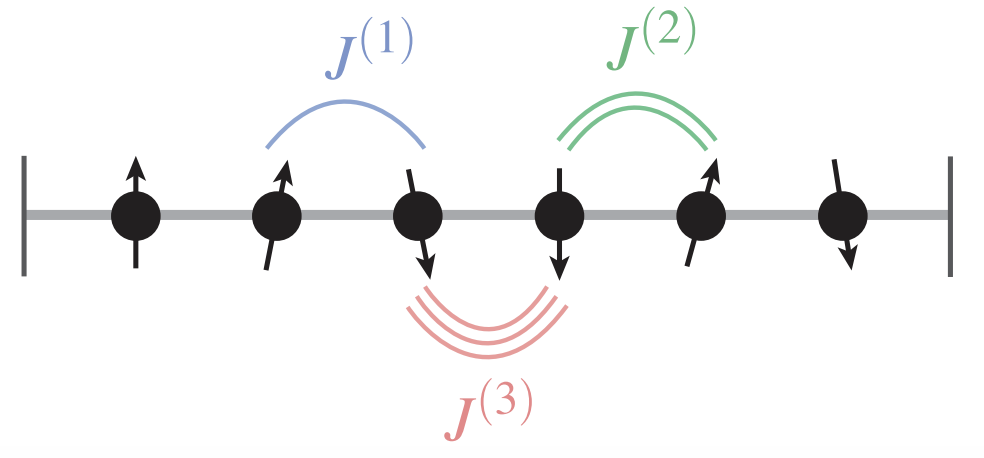
\includegraphics[width=0.5\textwidth]{fig/lattice.png}
	\caption{}
	\label{fig:chain}
\end{figure}

In the case of QMBT, one would like to understanding what phases of matter arise 
from strongly interacting quantum degrees of freedom. This is an interesting 
question because those phases display exotic properties desirable for, say, 
quantum computing applications, and because theses phases afford us insight 
into deep aspects of quantum field theory generally. The fact that the degrees 
of freedom are strongly interacting makes this in general a challenging task. 
Typically these systems are situated on a \textbf{lattice}---a
grid\footnote{Technically it does not have to be a square grid, it can be for instance
a tiling of triangles with degrees of freedom at every vertex.} of points 
which may represent, say, the atoms of a crystal. We can work with lattices 
in any dimension, but for simplicity this project will focus on one-dimensional 
lattices (referred to as chains). We refer to the points on the grid as 
\textbf{sites}, and of things occurring on a particular site or on a group of 
nearby sites as \textbf{local}.

What are the degrees of freedom on the lattice? In principle can be anything: 
discrete, continuous, multivalued, etc. In the case of (strongly interacting)
quantum matter usually it is something called the \textbf{spin}. Every electron
comes with a small magnetic moment which, when measured, points in one of two
directions (we can think of them as up or down). Of course, since this is
quantum physics, the electrons can also be in a superposition of the up and down
state; nonetheless, when we make a measurement we only find them in one of these
two configurations. Electrons' spins might interact with one another such that
the spins tend to align, or perhaps anti-align; thus, we have a strongly
interacting quantum system on a chain, see \cref{fig:chain}.

We represent the state that the system can be found in as a complex-valued
vector called the \textbf{wavefunction}. For instance, for the spin of one
electron, we might have a wavefunction 
\begin{equation*}
	\ket{\psi} = \begin{bmatrix}
	\alpha \\ \beta
	\end{bmatrix}
\end{equation*}
The notation on the left is called bra-ket notation. In that notation vectors 
are represented by $ \ket{} $ and transposed vectors by $ \bra{} $ (note this 
is the conjugate transpose, so we also take the complex conjugate). An inner 
product is then $ \braket{\psi\vert\phi} $. The wavefunction represents, roughly, 
the probability that the system is found in a particular state upon observation. More 
precisely, the absolute value squared represents the probability. For instance, 
consider the up state: 
\begin{equation*}
	\ket{\uparrow}= \begin{bmatrix}
	1\\0
	\end{bmatrix},\qquad 
	|\braket{\uparrow\mid\psi}|^2 = |\alpha|^2
\end{equation*}
A down state can be written similarly as $ \ket{\downarrow} = (0, 1) $. 

Observable quantities of a quantum-mechanical system are referred to as 
\textbf{observables}; they are represented by matrices. The expectation value 
of an observable is calculated by the inner product $ \bra{\psi}A\ket{\psi} $
and is denoted $ \langle A \rangle $. One very important observable is the 
\textbf{Hamiltonian}, denoted $ H $, which is nothing more than the energy of the system. 
It contains the particular interactions the system experiences---for instance, 
whether the spins tend to align, or whether they are reacting to magnetic field, etc.
It is an important observable because how the system changes over time turns 
out to be entirely dependent on the Hamiltonian. In fact, the states of the 
system that \textit{don't change} in time are the eigenvectors of the Hamiltonian 
(called eigenstates); their energies are the eigenvalues. The lowest-energy
eigenstate, termed the \textbf{ground state}, is taken to be the most important 
state, as we find that it describes the state the system will tend to settle 
in under typical circumstances, and thus captures the properties of that particular 
phase of matter. Generally, we know the Hamiltonian for the system but not the 
ground state; thus, finding the ground state wavefunction is more or less the 
main aim of quantum mechanics problems.

We have considered a wavefunction for one spin. For many spins, one must 
combine the wavefunctions by taking \href{https://en.wikipedia.org/wiki/Kronecker_product}{tensor products}.
The wavefunction will then be a vector of size $ 2^{N} $, where $ N $ is the 
number of electrons/lattice sites. 
This exponential growth makes it very difficult 
to find the eigenvectors of the Hamiltonian (and thus the ground state) by 
brute force algorithms as one runs out of memory quickly. It is referred to as
the curse of dimensionality. The bulk of computational QMBT is dedicated to
circumventing this bottleneck:
in order to solve a Hamiltonian for a significant number of particles, one
needs to be cleverer.

The many-body wavefunction can be written as 
\begin{equation*}
	\ket{\psi} = \sum_{\left\{\sigma_{i}\right\}} \psi(\sigma_1, \dots, \sigma_N)
	\ket{\sigma_1, \dots, \sigma_N}
\end{equation*}
here $ \sigma_i $ represents the spin of the electron on the $ i $-th site, 
and $ \ket{\sigma_1 ,\dots, \sigma_N} $ is a basis vector for a particular 
spin configuration (e.g., $ \ket{\uparrow, \downarrow, \dots\downarrow } $).
$ \left\{\sigma_i\right\} $ denotes a sum over all possible configurations of 
spins.  $ \psi(\sigma_1,\dots,\sigma_N) $ is the complex number representing the
value of that entry of the wavefunction vector. Since figuring out a basis is 
easy (we just need to list out every combination of up and down spins), 
the task lies in finding $ \psi(\sigma_1, \dots,\sigma_N) $.


\section{(Restricted) Boltzmann Machines}
\begin{figure}[t]
	\centering
	\begin{subfigure}[b]{0.45\textwidth}
		\centering
		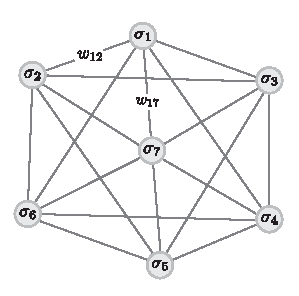
\includegraphics[width=\textwidth]{fig/boltzmann.pdf}
		\caption{Boltzmann machine.}
		\label{fig:boltzmann}
	\end{subfigure}
	\begin{subfigure}[b]{0.45\textwidth}
		\centering
		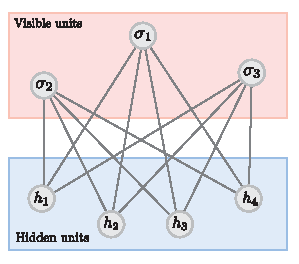
\includegraphics[width=\textwidth]{fig/restricted-boltzmann.pdf}
		\caption{Restricted Boltzmann machine. $ h_i $ do not connect to other 
		$ h_i $ and likewise for $ \sigma_i $.}
		\label{fig:restricted-boltzmann}
	\end{subfigure}
	\caption{}
\end{figure}

Boltzmann machines are a type of neural network which leverage insights from 
statistical physics to perform unsupervised learning of probabilistic models. 
That is, the goal is to use the Boltzmann machine to learn some target 
probability distribution $ p_{\text{T}}(X) $ given samples drawn from that 
probability distribution. 

The machine itself consists of a set of units $ \sigma_i $ and weights $ w_{ij} $
connecting each of those units (\cref{fig:boltzmann}). One defines an energy 
function 
\begin{equation}
	E(\sigma; w_{ij}, a_i) = \sum_i a_i \sigma_i + \sum_{ij} \sigma_i w_{ij} \sigma_j
\end{equation}
with biases $ a_i $ and weights $ w_{ij} $ connecting each unit to every other 
unit. The units themselves are binary with $ \pm 1 $ (some other authors choose $ 
\left\{0,1\right\} $). This model belongs to the class of \textbf{energy-based 
models}; such models leverage the fact that for an appropriately chosen 
$ E(v) $ (in the Boltzmann machine case, appropriately chosen $ w_{ij} $)
the target probability distribution---call this $ p_{\text{T}}(\sigma) $---can be
sufficiently approximated by the Boltzmann distribution
\begin{equation*}\label{eq:boltzmann-machine-distribution}
	p(\sigma) = \frac{1}{Z} e^{-E(\sigma; w_{ij}, a_i)}
\end{equation*}
where 
\begin{equation*}
	Z = \sum_{\left\{\sigma_i\right\}} \exp(-E (\sigma_i; w_{ij}, a_i))
\end{equation*}
is the partition function, i.e., the sum over all possible $ \sigma_i $ 
configurations that functions as a normalizing constant.

The model then trains $ w_{ij} $ by minizing some sort of measure of the 
divergence of $ p(\sigma) $ from $ p_{\text{T}}(\sigma) $---for instance 
maximum likelihood estimation or the Kullbach-Leibler divergence. Thus, given 
an unlabelled dataset $ \left\{\vbg{\upsigma}_n\right\} $ which is drawn 
from the unknown distribution $ p_{\text{T}} $, we may find $ E(\sigma; w_{ij},
a_i) $ such that $ p(\sigma) $ approximates $ p_{\text{T}} $. 

In practice, however, it is quite difficult to sample $ p(\sigma) $ for 
training purposes. The culprit is $ Z $, whose difficulty to evaluate is
well-known to physicists. One then resorts to the usual techniques employed 
to evaluate complex sums or integrals of this kind---chiefly, Monte Carlo
methods. We will see that the training of neural quantum states is no
different and we will need to employ Monte Carlo sampling of the wavefunction.

A special case of the Boltzmann machine that was designed with training
convenience in mind is the \textbf{restricted Boltzmann machine}. A restricted 
Boltzmann machine demotes a subset of $ \sigma_i $ to hidden units denoted $ h_i
$---these are units which do not appear as arguments to the probability
distribution $ p(\sigma_i) $ and whose purpose is analogous to a hidden layer 
in a feedforward network. Further, and crucially, we stipulate that the 
hidden units do not connect to themselves, only to visible units, and likewise 
for visible units (\cref{fig:restricted-boltzmann}). This amounts to writing $
\sigma_i w_{ij} \sigma_j$ as $ h_i w_{ij} \sigma_j $, so that 
\begin{equation*}
	E(\sigma_i; w_{ij}, a_i, b_i)
		= \sum_i a_i \sigma_i + \sum_i b_i h_i + \sum_{ij} h_i w_{ij} \sigma_j
\end{equation*}
(we have separated the bias into a visible bias $ a_i $ and a hidden bias 
$ b_i $).
The target probability distribution is approximated by the marginalization 
over $ h_i $---the trace, in physics parlance---so we must sum over $ h_i $
\begin{equation*}
	p(\sigma_i) 
		= \sum_{\left\{h_i\right\}} e^{-E(\sigma, h)}
\end{equation*}
The gradient (of the log) for the $ n $-th vector $ \vbg{\upsigma}_n $
\begin{align*}
	\frac{\partial \log p(\hat{\vbg{\upsigma}}_n)}{\partial w_{ij}}
		= \frac{1}{p(\hat{\vbg{\upsigma}}_n)} \frac{\partial p(\hat{\vbg{\upsigma}}_n)}{\partial w_{ij}}
		= \frac{1}{p(\hat{\vbg{\upsigma}}_n)} \left[
			\sum_{\left\{h_i\right\}} e^{-E(v,\hat{\vbg{\upsigma}}_n)} 
			\frac{\partial }{\partial w_{ij}} \left(\frac{1}{Z}\right) 
			+ \frac{1}{Z} \sum_{\left\{h_i\right\}} \frac{\partial }{\partial w_{ij}}
				e^{-E(h, \hat{\vbg{\upsigma}}_n)}
		\right]
		\\ 
		= \frac{1}{Z}\frac{1}{p(\hat{\vbg{\upsigma}}_n)} \left[
			-\sum_{\left\{h_i\right\}} e^{-E(v,\hat{\vbg{\upsigma}}_n)} \frac{1}{Z^2} \frac{\partial Z }{\partial w_{ij}} 
			- \frac{1}{Z} \sum_{\left\{h_i\right\}} 
			e^{-E(h, \hat{\vbg{\upsigma}}_n)} \hat{\sigma}_{n,i} h_j
			\right]
\end{align*}
The derivative of the partition function is 
\begin{align*}
	\frac{\partial Z}{\partial w_{ij}}
		= \frac{\partial }{\partial w_{ij}} 
			\sum_{\left\{h_i\right\}}
			\sum_{\left\{\sigma_i\right\}}
			e^{-E(h, \vbg{\upsigma}_n)}
		= \sum_{\left\{h_i\right\}}
			\sum_{\left\{\sigma_i\right\}}
			e^{-E(h, \vbg{\upsigma}_n)}
			(-\sigma_i, h_j)
		= - Z \langle \sigma_i v_j \rangle_{\text{model}}
\end{align*}
The subscript ``model'' says that this is the expectation value of the 
current forward pass Boltzmann machine distribution as opposed to the 
expectation value with respect to the data, which will show up shortly. 
Then we have 
\begin{align*}
	\frac{\partial \log p(\hat{\vbg{\upsigma}}_n)}{\partial w_{ij}}
		&= \frac{1}{p(\hat{\vbg{\upsigma}}_n)} \Bigg[
			\overbrace{\frac{1}{Z}\sum_{\left\{h_i\right\}} e^{-E(v,\hat{\vbg{\upsigma}}_n)}}^{p(\hat{\vbg{\upsigma}})}
			\frac{Z}{Z} \langle \sigma_i h_j \rangle_{\text{model}}
			- \overbrace{\frac{1}{Z} \sum_{\left\{h_i\right\}} 
			e^{-E(h, \hat{\vbg{\upsigma}}_n)}}^{p(\hat{\vbg{\upsigma}})}
			 \hat{\sigma}_{n,i} h_j
			\Bigg]\\
		&= \langle \sigma_i h_j \rangle_{\text{model}} 
			- \hat{\sigma}_{n,i} h_j
\end{align*}
Now, the gradient is the expected value over the training vectors $ \hat{\vbg{\upsigma}}_n $, 
so the derivative is
\begin{equation*}
	\frac{\partial \log p(\hat{\vbg{\upsigma}}_n)}{\partial w_{ij}}
	= \langle \sigma_i h_j \rangle_{\text{model}} 
		- \langle\hat{\sigma}_{n,i} h_j\rangle_{\text{data}}.
\end{equation*}
The benefit of the restricted Boltzmann machine is that there is an exact 
distribution that $ h_j $ follows given some $ \hat{\upsigma}_n $, so we 
can evaluate the second term. Let's say that $ h_k\in\left\{0,1\right\} $; 
the probability that $ h_k = 1$ given a visible unit can be calculated as follows. 
We have 
\begin{equation*}
	\frac{p(h_k=1\mid \sigma)}{p(h_k=0\mid \sigma)}
		= \frac{
			\exp\left[b_k + \sum_{i\neq k h_i b_i} + \sum_i v_i a_i + \sum_{i\neq k, j}h_i w_{ij} v_j
				+ \sum_j w_{kj} v_j\right]
		}{
			\exp\left[0\cdot b_k + \sum_{i\neq k h_i b_i} + \sum_i v_i a_i + \sum_{i\neq k, j}h_i w_{ij} v_j
				+ 0\cdot \sum_j w_{kj} v_j\right]
		}
\end{equation*}
Now, since $ h_k $ can only be in two states, $ p(h_k = 0\mid \sigma) = 1- p(h_k 0\mid\sigma)$, and 

\begin{align*}
	\frac{p(h_k=1\mid \sigma)}{1-p(h_k=1\mid \sigma)}
		&= \frac{
			\exp\left[b_k + \sum_{i\neq k h_i b_i} + \sum_i v_i a_i 
			+ \sum_{i\neq k, j}h_i w_{ij} v_j
				+ \sum_j w_{kj} v_j\right]
		}{
			\exp\left[\sum_{i\neq k h_i b_i} + \sum_i v_i a_i 
			+ \sum_{i\neq k, j}h_i w_{ij} v_j\right]
		}
		\\
		&=\exp\left(b_k + w_{kj} v_j\right)
\end{align*}
We can work out
\begin{equation*}
	p = e^W (1-p) \Longrightarrow (1+e^W) = e \Longrightarrow 
	p = \frac{e^W}{1 + e^W } \Longrightarrow \frac{1}{1+e^{-W}} = \sigma(-W)
\end{equation*}
So that the above implies
\begin{equation*}
	p(h_k = 1\mid \sigma) = \sigma(b_k + \sum_{j} w_{kj}v_j).
\end{equation*}
Notice that the argument relies on the fact that $ h_i $ does not connect 
to other hidden units. An identical argument finds 
\begin{equation*}
	p(\sigma_k = 1 \mid h) = \sigma(a_k + \sum_j w_{jk} )
\end{equation*}
Sampling $ \langle \sigma_i h_j\rangle_{\text{model}} $, however, remains
difficult. Strategies for doing so that leverage $ p(h_k=1\mid \sigma) $ and 
$ p(\sigma_k = 1\mid h) $ are described in Hinton. In the case of neural quantum 
states, however, the natural loss function is the energy of the system, and 
the gradients we must calculate are not the above. The evaluation will still 
be difficult, but in this case only because we must obtain the energy and its 
gradients indirectly in order to circumvent the curse of dimensionality. 

\section{Neural Quantum States}
One can view the many-body wavefunction $ \psi(\sigma_1, \dots, \sigma_N) $ 
appearing in 
\begin{equation*}
	\ket{\psi} = \sum_{\left\{\sigma_i\right\}} \psi(\sigma_1, \dots,\sigma_N)
		\ket{\sigma_1,\cdots, \sigma_N }
\end{equation*}
as a function from local degrees of freedom to a complex number, the amplitude, 
$ \psi : \left\{\sigma_i\right\} \to \C $. Thus we may treat $ \psi $ as a 
a Boltzmann machine with visible units $ \left\{\sigma_i\right\} $, albeit 
one that produces a complex number corresponding to the wavefunction as opposed 
to the probability amplitude. We thus provide $ \psi $ with a set of weights 
$ W = (w_{ij}, a_i, b_i)$ and hidden units $ h_i $ such that 
\begin{equation*}
	\psi(\sigma_1, \dots, \sigma_N; W)
		= \sum_{\left\{h_i\right\}}
			\exp\left(\sum_j a_j \sigma_j^z + \sum_i b_i h_i 
					+\sum_{ij} w_{ij} h_i \sigma_j^z \right)
\end{equation*}
Because $ \psi $ is complex-valued, $ w_{ij} $, $ a_i $, $ b_i $ are likewise 
taken to be complex valued. This is a restricted Boltzmann machine; we thus 
can explicitly marginalize $ \psi $:
\begin{align*}
	\psi 
		&= \sum_{\left\{ h_i \right\}}
			\exp\left(\sum_j a_j \sigma_j^z + \sum_i b_i h_i 
					+\sum_{ij} w_{ij} h_i \sigma_j^z \right)\\
	    &= \sum_{\left\{ h_i \right\}}
			\exp\left(\sum_j a_j \sigma_j^z\right) 
			\prod_i^M \exp\left(\sum_i b_i h_i\right) 
						\exp\left(\sum_j w_{ij} h_i \sigma_j^z\right)
\end{align*}
where we move the summation into the product as follows: 
\begin{align*}
	&= \exp \left( \sum_j a_j \sigma_j^z \right)
		\prod_i^M \sum_{h_i = \left\{ \pm 1 \right\}} 
			\exp\left(\sum_i b_i h_i\right)
			\exp\left(\sum_{ij} w_{ij} h_i \sigma_j^z\right) 
	\\ 
	&= \exp\left(\sum_j a_j \sigma_j^z \right)
	\prod_i^M \left[
		\exp\left(b_i + \sum_j w_{ij} \sigma_j^z \right)
		+ \exp\left(-b_i - \sum_j w_{ij} \sigma_j^z \right)
	\right]
	\\
	&= \exp\left(\sum_j a_j \sigma_j^z \right)
		\prod_i^M 2\cosh\left(b_i +\sum_{j} w_{ij} \sigma_j^z\right)
\end{align*}

\begin{thinnamedbox}[Note]
For some reason I always have to convince myself that the above move works, 
so for future reference here's the argument: we have a product indexed by 
$ i $ and a sum indexed by $ \ell $, which expanded looks like
\begin{align*}
	\prod_i^I \sum_\ell^L a_{i\ell}
		&= (a_{11} + a_{12} + \cdots + a_{1L})\\[-1em]
		&\qquad \times (a_{21} + \cdots + a_{2L})\\
		&\qquad \cdots \times (a_{I1} + \cdots + a_{IL})
\end{align*}
If we expand the products of sums, we obtain 
\begin{equation*}
	= a_{11} a_{21}\cdots a_{I1} + \cdots + a_{1L} a_{2L} \cdots a_{IL}
	= \sum_{a_{1i}}^L
	 \sum_{a_{2i}}^L \cdots
	 \sum_{a_{Li}}^L 
	 \prod_i^I a_{i\ell}.
\end{equation*}

\end{thinnamedbox}

Thus 
\begin{equation*}
	\psi(\sigma_1, \dots, \sigma_N; W)
	= 
	\exp\left(\sum_j a_j \sigma_j^z \right)
	\prod_i^M 2\cosh\left(b_i +\sum_{j} w_{ij} \sigma_j^z\right)
\end{equation*}

Given a Hamiltonian $ H $, how do we update $ w_{ij} $, $ a_i $, $ b_i $
to minimize the energy $ H = \bra{\psi}H\ket{\psi} $? As is typical with 
this type of problem, one resorts to a Monte Carlo method. Carleo and Troyer 
use a technique called stochastic reconfiguration wherein one updates the 
weights as 
\begin{equation*}
	W_{k+1, i}= W_{k,i} - \gamma_k S^{-1}_{k, ij} F_{k, j}
	\qquad (k=\text{iteration step})
\end{equation*}
where 
\begin{gather*}
	S_{k,ij} = \langle O_i^\dagger O_j\rangle - \langle O_i^\dagger\rangle \langle O_j\rangle,\qquad 
	F_{i} = \langle E_{\text{loc}} O_i^\dagger\rangle - \langle E_{\text{loc}}\rangle
		\langle O_i^\dagger \rangle\\
	O_i = \frac{1}{\psi} \partial_{W_i} \psi,\qquad 
	E_{\text{loc}} = \frac{1}{\psi}\bra{\left\{\sigma_i\right\}} H \ket{\psi} 
\end{gather*}
Here the expectation values denote $ \langle A\rangle = \sum_{\left\{\sigma_i\right\}} 
A (\left\{\sigma_i\right\})|\psi(\left\{\sigma_i\right\})|^2 $. They are 
evaluted with a Markov chain sampled with a Metropolis-Hastings procedure:
as is common with these VMC techniques, we flip a random spin and accept the 
new configuration with probability 
\begin{equation*}
	P(\left\{\sigma_i\right\}_k \to \left\{\sigma_i\right\}_{k+1})
		= \min \left(1, \Bigg| \frac{
				\psi(\left\{\sigma_i\right\}_{k+1})
			}{
				\psi(\left\{\sigma_i\right\}_{k})}\Bigg|^2\right).
\end{equation*}

\subsection*{References}
\begin{itemize}[itemsep=0.2ex]
\item Giuseppe Carleo, Matthias Troyer, \textit{Solving the quantum many-body problem
with artificial neural networks}. Science 355, 602-606 (2017).
\href{https://doi.org/10.1126/science.aag2302}{DOI:10.1126/science.aag2302}. 
See the supplemental materials for information on their Monte Carlo sampling.
\item Torlai, Giacomo, and Roger G. Melko. \textit{"Learning thermodynamics with
Boltzmann machines."} Physical Review B 94.16 (2016): 165134.
\href{https://doi.org/10.1103/PhysRevB.94.165134}{DOI:10.1103/PhysRevB.94.165134}.
\item Grathwolh, et al., \textit{Your Classifier is Secretly an Energy Based Model and You Should Treat it Like One} (2019).
 \href{https://arxiv.org/abs/1912.03263}{arXiv:1912.03263}.
\item Hinton, \textit{A Practical Guide to Training
Restricted Boltzmann Machines}. \url{https://www.cs.toronto.edu/~hinton/absps/guideTR.pdf}.
\item Sorella, \textit{Green Function Monte Carlo with Stochastic Reconfiguration},
 \href{https://journals.aps.org/prl/abstract/10.1103/PhysRevLett.80.4558}{DOI:10.1103/ PhysRevLetter.80.5668}.
\end{itemize}


\end{document}